\def\year{2022}\relax
%File: formatting-instructions-latex-2022.tex
%release 2022.1
\documentclass[letterpaper]{article} % DO NOT CHANGE THIS
\usepackage{aaai22}  % DO NOT CHANGE THIS
\usepackage{times}  % DO NOT CHANGE THIS
\usepackage{helvet}  % DO NOT CHANGE THIS
\usepackage{courier}  % DO NOT CHANGE THIS
\usepackage[hyphens]{url}  % DO NOT CHANGE THIS
\usepackage{graphicx} % DO NOT CHANGE THIS
\urlstyle{rm} % DO NOT CHANGE THIS
\def\UrlFont{\rm}  % DO NOT CHANGE THIS
\usepackage{natbib}  % DO NOT CHANGE THIS AND DO NOT ADD ANY OPTIONS TO IT
\usepackage{caption} % DO NOT CHANGE THIS AND DO NOT ADD ANY OPTIONS TO IT
\DeclareCaptionStyle{ruled}{labelfont=normalfont,labelsep=colon,strut=off} % DO NOT CHANGE THIS
\frenchspacing  % DO NOT CHANGE THIS
\setlength{\pdfpagewidth}{8.5in}  % DO NOT CHANGE THIS
\setlength{\pdfpageheight}{11in}  % DO NOT CHANGE THIS
%
% These are recommended to typeset algorithms but not required. See the subsubsection on algorithms. Remove them if you don't have algorithms in your paper.
% \usepackage{algorithm}
% \usepackage{algorithmic}

%
% These are are recommended to typeset listings but not required. See the subsubsection on listing. Remove this block if you don't have listings in your paper.
% \usepackage{newfloat}
% \usepackage{listings}
% \lstset{%
% 	basicstyle={\footnotesize\ttfamily},% footnotesize acceptable for monospace
% 	numbers=left,numberstyle=\footnotesize,xleftmargin=2em,% show line numbers, remove this entire line if you don't want the numbers.
% 	aboveskip=0pt,belowskip=0pt,%
% 	showstringspaces=false,tabsize=2,breaklines=true}
% \floatstyle{ruled}
% \newfloat{listing}{tb}{lst}{}
% \floatname{listing}{Listing}

% User packages
\usepackage{amssymb}
\usepackage{booktabs}
\usepackage{mathtools}
\usepackage{bbm}  
% \usepackage[ruled,vlined,linesnumbered,noend]{algorithm2e}
\usepackage[ruled,vlined,linesnumbered]{algorithm2e}

\nocopyright

% ------
% User defined commands
\DeclareMathOperator*{\argmin}{arg min}      % argmin
\DeclareMathOperator*{\argmax}{arg max}      % argmin
\DeclarePairedDelimiter{\ceil}{\lceil}{\rceil}
\newcommand{\CC}{C\texttt{++}}
% ------

\pdfinfo{
/Title (An Analysis of Partial Pathfinding using Map Abstraction and Refinement)
/Author (Jake Tuero)
/TemplateVersion (2022.1)
}

% \setcounter{secnumdepth}{0}
\setcounter{secnumdepth}{1}

\title{An Analysis of Partial Pathfinding using Map Abstraction and Refinement} 
\author{
    Jake Tuero
    \\
}
\affiliations{
    Department of Computing Science, University of Alberta \\
    Edmonton, Canada\\
    tuero@ualberta.ca
}

\begin{document}

\maketitle


\begin{abstract}
A* provides a way of finding optimal paths over graphs.
However, the search cost of A* is greatly effected by the size of the search space,
and must wait for a complete path to be found before actions can be carried out in the environment.
This report investigates the PRA*($\infty$) and PRA*($k$) algorithms, their properties, and how they compare to A*.
\end{abstract}

\section{Introduction}
Pathfinding over grid-based environments has been well studied for decades,
as its applications has many uses such as in video game AI.
Traditional search algorithms find a complete path from start to goal
before an agent can begin to carry out those actions.
However, the environment may be dynamic which results in many replanning steps,
and there may not be enough compute time to find a full path before an action must be carried out.

Abstractions can be used to shrink the size of the search space, 
which directly decreases the time-to-completion for traditional search algorithms.
Ideally, these abstractions should have an automated way of forming such that changes in the environment can easily be dealt with.
This report investigates the PRA*($\infty$) and PRA*($k$) algorithms \cite{sturtevant2005partial},
which allows for fine-control over search speed, quality, and time-to-act in the environment.
We identify how these properties relate to each other 
through empirical experimentation over a wide variety of grid-based maps from popular video games.  
The rest of this paper is organized as follows:
a description of the problem PRA*($\infty$) and PRA*($k$) solves, and previous methods are introduced.
The PRA*($\infty$) and PRA*($k$) algorithms are formalized, and suitable properties to be tested are explained.
Finally, we demonstrate these properties and tradeoffs as compared to A* over a wide variety of scenarios.



\section{Background and Related Work}

\subsection*{The Pathfinding Problem}
The pathfinding problem can be described as finding a minimal cost path over a connected graph $G=(V,E)$,
where $G$ is the graph represented by the vertex set $V$ and edge set $E$.
Vertices are sets of nodes representing states in the environment,
and directed edges join neighbouring states $(s_1, s_2)$ if $s_2$ can be reached from $s_1$ by a single action.
Edges have an associated non-negative weight, which defines the cost of going from one neighbour to the next.
A \textit{path} is a sequence of actions which traverse from one node to the next,
and the \textit{cost} of that path is the sum of action costs (i.e. the sum of edge weights which the path covers).
A \textit{minimal cost} or \textit{optimal} path is a path such that no other path exists from the same start to goal node
which has a lower associated cost.

\subsection{The A* Algorithm}
A* \cite{hart1968formal} is a \textit{best-first} search algorithm which operates over graphs. 
The algorithm iteratively expands nodes of minimal $f$-cost from a priority queue,
adding children nodes (neighbours) into the queue,
until the goal node is reached.
The priority $f$-cost is defined as $f(n) = g(n) + h(n)$ for all nodes $n$,
where $g(n)$ is the path cost from the start node to $n$,
and $h(n)$ is a \textit{heuristic} estimate of the \textit{cost-to-go} from $n$ to the goal node.
The heuristic acts as guidance to the A* algorithm,
to prioritize states which are closer to the goal, reducing the overall search effort.

To ensure that optimal paths are found by the A* algorithm, 
there are some restrictions that must be placed on the heuristic $h$.
We denote $h^*(n)$ as the true minimal cost to a goal starting from node $n$.
A heuristic $h$ is \textit{admissible} if $h(n) \le h^*(n)$ for all $n$,
and is \textit{consistent} if $h(n) \le c(n, n') + h(n')$ for all pairs of nodes $n$ and $n'$,
where $c(n, n')$ is the minimal sum of edge costs between nodes $n$ and $n'$.

\subsection*{Pathfinding with Abstractions}
A* search's performance cost characteristics are directly related to the size of the graph which is being searched over.
Any abstractions which can be made to reduce the size of the graph which A* searches over can over speed-up improvements,
albeit at potentially not offering optimality.
One such automated way creating abstractions is the STAR abstraction \cite{holte1996speeding},
which represents abstract nodes as connected subgraphs containing all nodes within $R$ distance of a given node.
This can be done in an automated way, while providing granularity over level of abstraction through the $R$ parameter.

Search algorithms have used various types of abstraction to replace the underlying graph being searched over,
while keeping the search algorithm the same for the most part.
Hierarchical A* \cite{holte1996hierarchical} builds a hierarchy of abstract spaces,
with the purpose using each hierarchy to compute heuristics to use in the layers below.
Many abstract searches are used for a single base-level search.
Hierarchical Pathfinding A* \cite{botea2004near} uses spatial information from the underlying graph to build its abstractions 
specifically for grid-based pathfinding.
A pre-processing step superimposes sectors on top of the tile grids,
and an abstract is created by placing nodes at sector entrances, intra-sector edges and inter-sector edges
which joins nodes in each sector, and the sectors together.
An abstract path is then found over this abstract representation,
and path smoothing techniques are used to recover a path over the original graph.

% \subsection*{Partial Pathfinding}
% One of the downsides to traditional search algorithms such as A* is that a full path must be found before 
% the agent can start to make moves in the environment.
% If the search space is large, and there is little time for the agent to move,
% then there may not be enough time to make any move as the full path has not been found yet.
% Additionally, if the environment changes while the agent is implementing the found path,
% then a complete replanning needs to be done.
% There is a large body of work for real-time search algorithms which tackle these issues.





\section{Approach}
In this section, we give an overview of our the various components of our method is detailed.

\subsection{Automated Search Graph Abstractions}
To reduce the search effort, we would like an automated way of creating abstractions for grid-based environments,
such that the abstraction can be updated to reflect local changes to the environment.
In grid-based pathfinding, the environment is discretized into tiles,
where each tiles is octile-connected to its eight surrounding neighbours.
The base level of abstraction is a graph where each tile is represented by a single abstract node,
edges join neighbouring abstract nodes if their tiles are joined either cardinally or diagonally.

A hierarchy of abstractions can then be automated using an abstraction function $\mathcal{A}(G_k) \to G_{k+1}$.
Each node in $G_k$ can only be abstracted into a single node in $G_{k+1}$,
and nodes $n_{k+1,i}, n_{k+1, j}$ in $G_{k+1}$ are neighbours if the set of nodes which $n_{k+1,i}$ represents 
shares an edge in the original graph with a node in the original graph from the set of nodes represented by $n_{k+1,j}$.

The process by which nodes from abstraction level $k$ are mapped to $k+1$ is referred to by \textit{Clique-Abstraction},
which is given in Algorithm ~\ref{alg:ca}.
Starting with the largest clique size of 4, 
the graph is scanned for nodes which form a clique. 
These nodes are then formed into an abstract node for the next level, and removed from further consideration.
This process is then repeated for cliques of size 3 and 2.
Nodes which are not part of a clique previously formed and are only neighbouring to one other node are referred to as \textit{orphans}.
Orphans are added to the set of nodes which the clique neighbouring it represents.
Finally, any remaining nodes are treated as a clique of size 1.

\begin{algorithm}[ht]
\caption{\texttt{AddCliques}$(l)$}
\label{alg:isclique}
\KwIn{Node set $N$, Abstract Graph $G_{k+1}$}
\DontPrintSemicolon
\For{set $(n_1, \dots, n_l) \in N$} {
    \If{$IsClique(n_1, \dots, n_l)$} {
    Add node $(n_1, \dots, n_l) \in G_{k+1}$\;
    Remove $(n_1, \dots, n_l) \in N$\;
    }
}
\end{algorithm}

\begin{algorithm}[ht]
\caption{\texttt{Clique-Abstraction}$(G_k)$}
\label{alg:ca}
\DontPrintSemicolon
\KwIn{Abstract Graph $G_k=(V_k, E_k)$}
\KwOut{Abstract Graph $G_{k+1}=(V_{k+1}, E_{k+1})$}
$N \gets G_k(N)$ \;
$\textbf{AddCliques(4)}, \textbf{AddCliques(3)}, \textbf{AddCliques(2)}$\;

\For{$n_i \in N$} {
    \If{$\textbf{IsOrphan}(n_i)$} {
        Add to clique\;
        Remove $n_i \in N$\;
    }
}
$\textbf{AddCliques}(1)$\;

\For{pair $(n_1, n_2) \in G_{k+1}(N)$} {
    \If{neighbours($n_1, n_2$)} {
    Add edge $(n_1, n_2) \in G_{k+1}$\;
    }
}
\end{algorithm}

This process allows for a simple, yet automated way of create a hierarchy of abstractions.
Before this can be used in a search, we need to define distances between abstract nodes.
The \textit{position} $(x, y)$ pair of an abstract state is the average of positions of all the underlying tiles it represents.
Distances between two abstract nodes is give by
\begin{equation}\label{eq:distances}
    \sqrt{2} \cdot \min \left( |\Delta x|, |\Delta y| \right) + | \ |\Delta x| - |\Delta y| \ |.
\end{equation}


\subsection{Partial-Refinement A*}

\begin{algorithm}[t]
\caption{\texttt{RefinePath}$(start, goal, path)$}
\label{alg:refine}
\DontPrintSemicolon
\Return{A*($start$, $goal$) subject to nodes in $path$}\;
\end{algorithm}

\begin{algorithm}[ht]
\caption{\texttt{PRA*}$(k)$}
\label{alg:pra}
\DontPrintSemicolon
\KwIn{Abstract Graph $G_k=(V_k, E_k)$}
\KwIn{start $s$, goal $g$, $k$}

$start \gets s, goal \gets g$\;
$l \gets \text{starting abstraction level}$\;
\While{true}{
$path \gets \varnothing$\; 
\For{abstraction level $i \in \{l, \dots, 0\}$} {
    $path \gets \textbf{RefinePath}$($path$, $start$, $goal$)\;
    $path \gets$ truncated to length $k$\;
    $goal \gets path[-1]$\;
}
\If{goal == g} {
    \textbf{break}\;
}
$start \gets goal$\;
}
\end{algorithm}

The PRA* algorithm is given in Algorithm \ref{alg:refine} and Algorithm \ref{alg:pra}.
PRA* works by searching over an abstract graph,
and using the abstract path to restrict the search done in the next layer closer to the original graph.
The results from a previous higher-level search provides an informed corridor as to where the lower-level search should concentrate on.
Since each layer is restricted to the superimposed path from above, the search in each layer should be relatively cheap.
Below, we give more detail to each of the processes in PRA*.

\subsection*{Choosing an Starting Abstraction Level}
Given an abstract hierarchical clique graph as described in the previous section,
a starting abstraction level needs to be picked. 
The lower the abstraction level, the larger the search space and thus more work required.
However, the resulting path will be more accurate as compared to the ground truth solution path at the grounded level.
While further studies can look into this tradeoff, we choose the middle abstraction layer as the starting point 
as a balance of granularity and speed.

\subsection*{Performing Search over the Abstract Graph}
Once a starting layer is selected (Algorithm \ref{alg:pra} line 2),
an iterative process searches down the abstraction layers, 
using the abstract path from the previous layer to concentrate the search effort in the next layer.
Algorithm \ref{alg:pra} lines 4 to 8 highlight this process.

A search is performed over the current abstract layer from the abstract start node which represents the start tile in the original graph,
to the abstract goal node which represents the goal tile in the original graph.
The search algorithm used here is A*, and the search is restricted to only the abstract nodes which are represented by the path found in the previous iteration.
In the first iteration, there is no restriction as there is no initial starting path.
Distances between nodes use Equation \ref{eq:distances}.
This process repeats until the final layer is reached, which represents the original grid-based graph.

Due to how the abstract graph was created, paths which contain nodes which represents the start tile and goal tile are guaranteed 
to represent a legal path using the abstract nodes which that paths represents in the next layer down.
This is due to the fact that each abstract node is made up of a clique of abstract nodes in the previous layer.
Since a clique represents a fully connected graph, any node in a clique is connected to any other node in the same clique;
and abstract nodes are neighbours if their underlying set of nodes share a connection, thus connectivity is guaranteed. 

\subsection*{Partial Refinement}
An enhancement is for partial refinement in scenarios where we would like to move sooner than it would take to find a full path.
Given an integer parameter $k$, the found path is truncated to length at most $k$ at each step in the refinement process.
This algorithm is referred to as PRA*$(k)$, and the original algorithm without partial refinement is denoted as PRA*$(\infty)$.

A few adjustments need to be made to the algorithm to ensure that a complete path from the original start to goal is eventually returned.
The refinement process is encapsulated in an outer loop, 
which continues until the goal found for the current complete refinement process matches the original goal.
During refinement, the path is truncated to length $k$, as show in Algorithm \ref{alg:pra} line 7.
Because the original goal may have been truncated, the new goal to search for in the abstract layer below is given by the tail of the previous path,
shown in Algorithm \ref{alg:pra} line 8.
Once the complete refinement process is complete, 
a path from the current start to the current goal (which may no longer be the original goal).
The entire refinement process then continues, with the new current start being the goal found in the previous refinement step,
and the goal being reset to the original goal (Algorithm \ref{alg:pra} line 11).
Once the refinement process ends with the tail of the path matching the goal in question, the PRA*$(k)$ algorithm is complete.



\section{Experiments and Results}

\subsection*{Experiments}
There are a few properties of PRA*$(k)$ which is to be examined as compared against A*.
The first is the tradeoff between the increase in search efficiency compared to the suboptimality introduced by searching over coarser abstraction levels.
Second, is to examine the same tradeoff but as the $k$ parameter of PRA*$(k)$ varies.
A smaller $k$ value should allow for shorter times between when the agent can start to move, but the the cost of less accurate paths.

\subsection*{Environments}
Grid-based maps from Baldur's Gate and Warcraft 3 \cite{sturtevant2012benchmarks} are used for the domains to search over.
Each map is represented as a binary 512x512 grid of pathable and non-pathable tiles.
For each map, multiple scenarios of start and goal tile pairs are randomly selected.
To ensure a wide variety of path types, 
several paths for each \textit{bucket} is chosen for bucket values of [0, 127],
where a path having length $l$ belongs to bucket $i$ if $i = \lfloor l / 4 \rfloor$.


\subsection*{Implementation Details}
The algorithms and environment are implemented in {\CC},
using the {\CC}20 standard.
The codebase is compiled using the \textit{GNU Compiler Collection} version 11.1.0.
All experiments were run on an Intel i9-7960X, with 128GB of memory running Ubuntu 20.04.
Because multiple threads are used to speed-up the experimentation,
with each thread given a separate problem instance,
the CPU time is recorded instead of the wall clock time.
For further details, see the attached code.


\subsection*{Results}
\begin{figure*}[h]
\centering
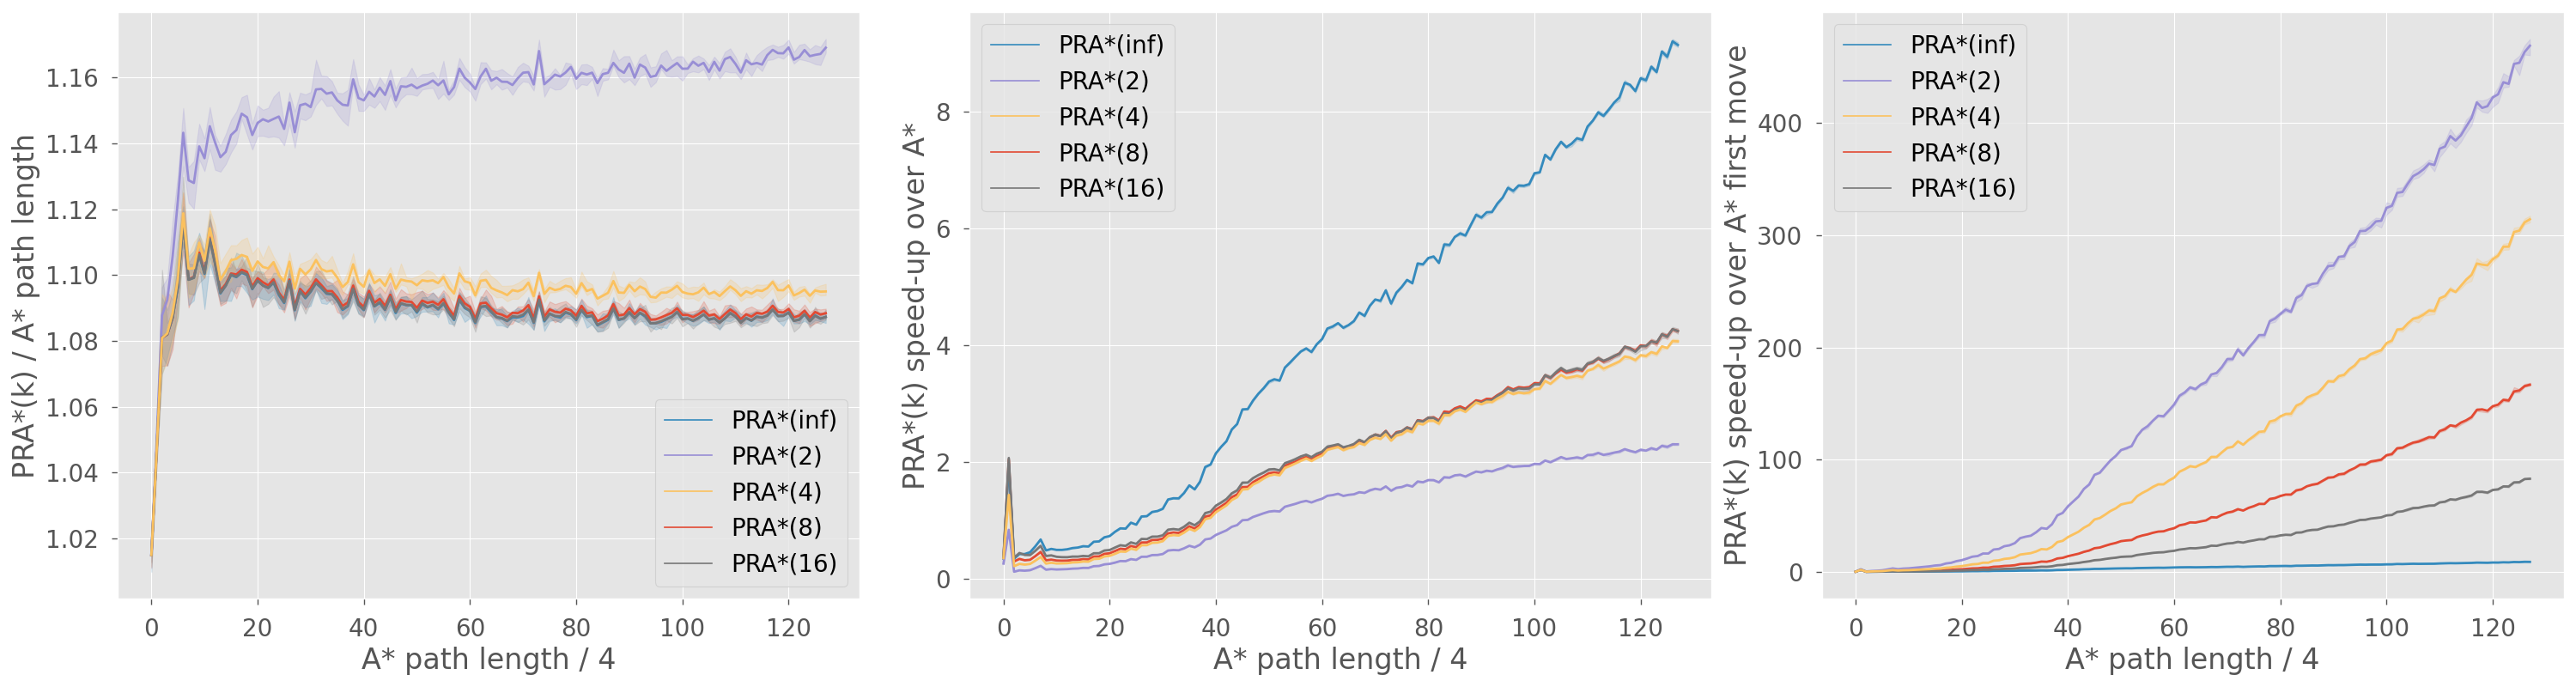
\includegraphics[width=0.85\paperwidth]{./assets/plot_combined.png}
\caption{
    PRA*($\infty$) and PRA*($k$) path quality and execution speed as compared to A*. 
    Lines show the average over all scenarios for its optimal path length, 
    with shaded regions showing the 95\% confidence intervals.
}
\label{fig_all}
\end{figure*}

Figure \ref{fig_all} shows the results of our experiments.
Figure \ref{fig_all}a) plots the path length found by PRA*($\infty$) and PRA*($k$) as a ratio to the path found by A*,
which is the optimal path length.
As the $k$ parameter value gets smaller, the paths found by PRA*($k$) increase in suboptimality.
This can be explained by each subsequent refinement step only having a partial path to the goal to work with;
as the path becomes smaller, less directional information is retained.

Figure \ref{fig_all}b) plots the speed-up provided by PRA*($\infty$) and PRA*($k$) as compared to the time it took for A* to find a path.
For PRA*($k$), the time used is the total time for all refinements steps to recover a path from the original start to the original goal.
PRA*($\infty$) offers the largest increase in speed as compared to A*, and carries this speed-up as the path length increases.
For smaller values of $k$, PRA*($k$) does not offer as large as a speed-up as compared to PRA*($\infty$).
This can be due to the fact that many refinement iterations need to be done, as only a short path is recovered for each outer iteration.

Finally, 
Figure \ref{fig_all}c) plots the speed-up provided by PRA*($\infty$) and PRA*($k$) 
in terms of returning a full or partial path 
at the grounded level such that the agent can start to move.
Faster turnaround times for returning an action sequence means that an agent following this path can plan and act in the environment interchangeably.
For smaller values of $k$, PRA*($k$) is able to provide a starting partial path which can start to be implemented much faster than PRA*($\infty$) and A*,
which must wait for the entire path from start to goal to be found before an action sequence can start to be implemented.

\section{Conclusion}
This report has provided an overview of the implementation of the PRA*($\infty$) and PRA*($k$) search algorithms,
and an empirical analysis of the properties and tradeoffs these algorithms provide.
Both PRA*($\infty$) and PRA*($k$) offer speed-up improvements over A*, at the cost of optimality.
PRA*($\infty$) offers paths closer to optimal with a moderate speed-up,
while PRA*($k$) allows for fast reactive planning and acting as partial paths are returned very quickly.
There were some details not looked at which should be considered for future work, 
namely looking at methods to determine what is the appropriate level of starting abstraction,
and how the parameter value $k$ is affected by this choice.


\bibliography{references}

\section*{Appendix}
For a brief guide on the layout of the codebase and where to find experimental runs, 
see the included \texttt{instructions.txt}.
For a more detailed guide, including compiling and helper script instructions,
see the \texttt{readme.md} file in the \texttt{pra} directory.

\end{document}
